% !TeX root = ../main.tex

% =================== 文獻探討 =================== %
\section{文獻探討}

\textbf{\textbackslash textbf\{要加粗的字\} 使字體加粗},
\underline{\textbackslash underline\{要加底線的字\} 加上底線},
\textit{\textbackslash textit\{要斜體的字\} 為斜體字,只是中文並不明顯,english is italic better}。

在內文中打\textbackslash\textbackslash 為強制\\換行。

空一行可以

換段(換段會縮排,換行不會)。僅用enter鍵到下一行
不會換段
也不會換行。(搭配sections/02related\_work.tex來看會更清楚)

可以用\textbackslash footnote\{註解寫在這裡\}在頁面底部加入註解\footnote{這是一個註解。},\footnote{註解會自動編號。}。

\textbackslash clearpage 可以強制
\clearpage
換頁。

% ------------------- 小標題 -------------------- %
\subsection{小標題}

論文引用使用\textbackslash cite\{這裡填論文在.bib中的label\} \cite{Rowe:2005:ASR};可以一次引用多篇論文 \cite{Rowe:2005:ASR,vinet1989universal}。

使用下方格式來插入圖片,使用\textbackslash ref\{label\}來引用圖 \ref{figure:fig1}。
\begin{lstlisting}[language=TeX]
    \begin{figure}[!htb]
        \centering
        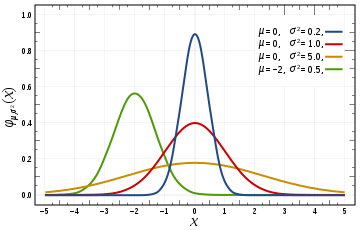
\includegraphics[width=0.5\textwidth]{figures/gambar.png}
        \caption{範例圖片}       % 圖片標題
        \label{figure:fig1}     % 圖片引用標籤
    \end{figure}
\end{lstlisting}
如果是使用1.docker環境或是2.local環境且有按造教學設定LaTeX\ Utilities的使用者,可以複製圖片的路徑,並在要插入圖片的位置按下Ctrl+Shift+V,即可自動產生插入圖片的程式碼。\\
如果發現圖片內容會被浮水印影響,可以使用\textbackslash colorbox\{white\}加上白底,如圖 \ref{figure:fig2}。

% ------------------- 小小標題 ------------------- %
\subsubsection{小小標題}

\begin{figure}[!htb]
    \centering
    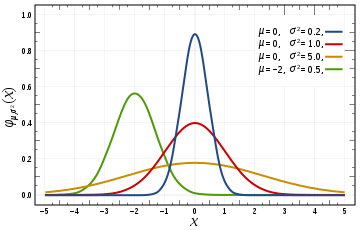
\includegraphics[width=0.5\textwidth]{figures/gambar.png}
    \caption{範例圖片}
    \label{figure:fig1}
\end{figure}

% 插入背景為白色的gamber.png
\begin{figure}[!htb]
    \centering
    \colorbox{white}{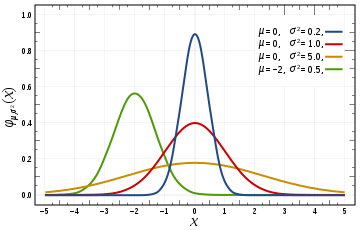
\includegraphics[width=0.5\textwidth]{figures/gambar.png}}
    \caption{範例白底圖片}
    \label{figure:fig2}
\end{figure}


% ------------------- 列點範例 ------------------ %
\subsection{列點範例}

\begin{itemize}
    \item 個別項目以黑點表示,稱為項目符號。
    \item 項目中的文字可以是任意長度。
\end{itemize}

\begin{enumerate}
    \item 這是清單中的第一個項目。
    \item 隨著每個新增的項目,清單編號會增加。
\end{enumerate}

\begin{enumerate} [leftmargin=3cm]      % 設定左邊距
    \item[第一章:] 可以自訂清單標籤。
    \item[第二章:] 這是一個自訂清單標籤的範例。
\end{enumerate}


% ------------------- 子圖範例 ------------------ %
\subsection{子圖範例}

三子圖範例,如圖 \ref{fig:three graphs};四子圖範例,如圖 \ref{fig:four graphs};
子圖之間可以無間格,如圖 \ref{fig:four_nospace};子圖可以不單獨寫標題,如圖 \ref{fig:four_nocaption}。

\begin{figure}[!htb]
    \centering
    \begin{subfigure}[b]{0.3\textwidth}
        \centering
        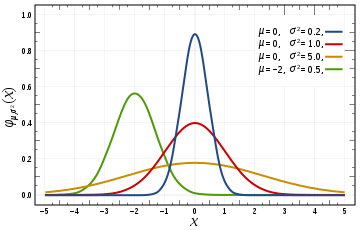
\includegraphics[width=\textwidth]{figures/gambar.png}
        \caption{$y=x$}
        \label{fig:y equals x}
    \end{subfigure}
    \hfill
    \begin{subfigure}[b]{0.3\textwidth}
        \centering
        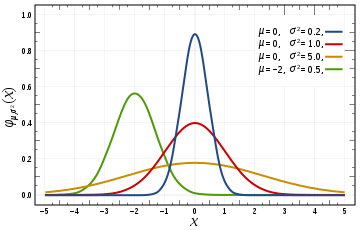
\includegraphics[width=\textwidth]{figures/gambar.png}
        \caption{$y=3\sin x$}
        \label{fig:three sin x}
    \end{subfigure}
    \hfill
    \begin{subfigure}[b]{0.3\textwidth}
        \centering
        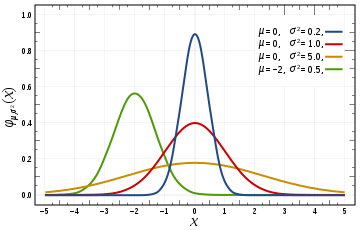
\includegraphics[width=\textwidth]{figures/gambar.png}
        \caption{$y=5/x$}
        \label{fig:five over x}
    \end{subfigure}
       \caption{三子圖範例}
       \label{fig:three graphs}
\end{figure}

\begin{figure}[!htb]
    \centering
    \begin{subfigure}{0.4\textwidth}
        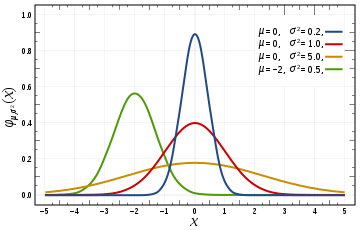
\includegraphics[width=\textwidth]{figures/gambar.png}
        \caption{Firts subfigure.}
        \label{fig:first}
    \end{subfigure}
    \hfill
    \begin{subfigure}{0.4\textwidth}
        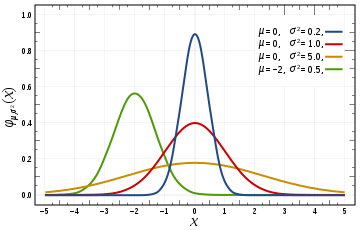
\includegraphics[width=\textwidth]{figures/gambar.png}
        \caption{Second subfigure.}
        \label{fig:second}
    \end{subfigure}
    \hfill
    \begin{subfigure}{0.4\textwidth}
        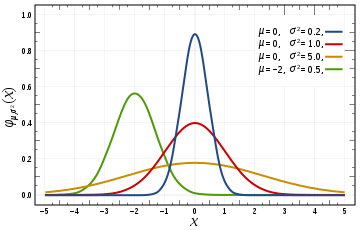
\includegraphics[width=\textwidth]{figures/gambar.png}
        \caption{Third subfigure.}
        \label{fig:third}
    \end{subfigure}
    \hfill
    \begin{subfigure}{0.4\textwidth}
        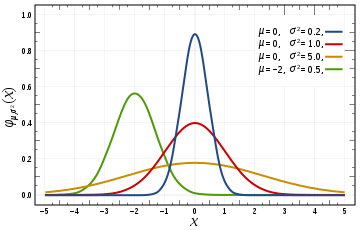
\includegraphics[width=\textwidth]{figures/gambar.png}
        \caption{Third subfigure.}
        \label{fig:fourth}
    \end{subfigure}
    \caption{四子圖範例}
    \label{fig:four graphs}
\end{figure}

\begin{figure}[!htb]
    \centering
    \begin{subfigure}{0.4\textwidth}
        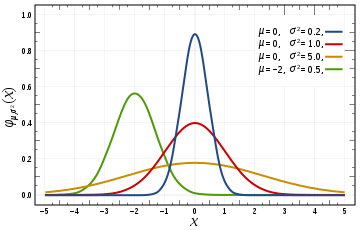
\includegraphics[width=\textwidth]{figures/gambar.png}
        \caption{Firts subfigure.}
        \label{fig:first_nospace}
    \end{subfigure}
    \begin{subfigure}{0.4\textwidth}
        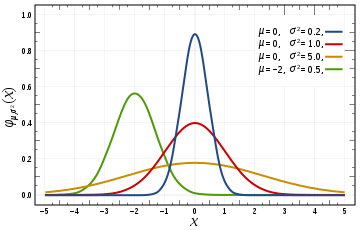
\includegraphics[width=\textwidth]{figures/gambar.png}
        \caption{Second subfigure.}
        \label{fig:second_nospace}
    \end{subfigure}
    \begin{subfigure}{0.4\textwidth}
        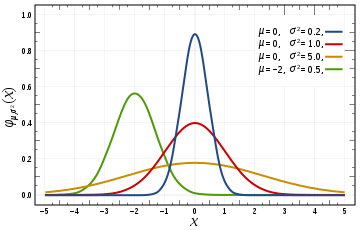
\includegraphics[width=\textwidth]{figures/gambar.png}
        \caption{Third subfigure.}
        \label{fig:third_nospace}
    \end{subfigure}
    \begin{subfigure}{0.4\textwidth}
        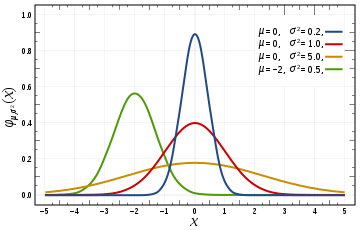
\includegraphics[width=\textwidth]{figures/gambar.png}
        \caption{Third subfigure.}
        \label{fig:fourth_nospace}
    \end{subfigure}
    \caption{無間格四子圖範例}
    \label{fig:four_nospace}
\end{figure}

\begin{figure}[!htb]
    \centering
    \begin{subfigure}{0.4\textwidth}
        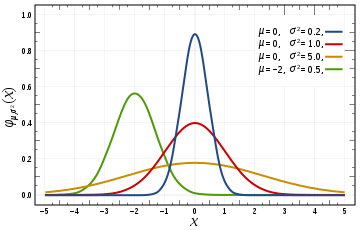
\includegraphics[width=\textwidth]{figures/gambar.png}
        \caption{}
        \label{fig:first_nocaption}
    \end{subfigure}
    \begin{subfigure}{0.4\textwidth}
        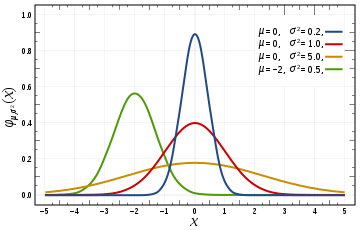
\includegraphics[width=\textwidth]{figures/gambar.png}
        \caption{}
        \label{fig:second_nocaption}
    \end{subfigure}
    \begin{subfigure}{0.4\textwidth}
        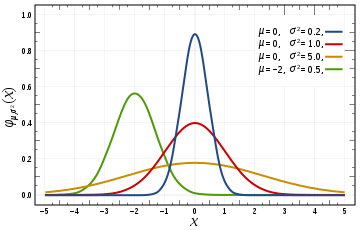
\includegraphics[width=\textwidth]{figures/gambar.png}
        \caption{}
        \label{fig:third_nocaption}
    \end{subfigure}
    \begin{subfigure}{0.4\textwidth}
        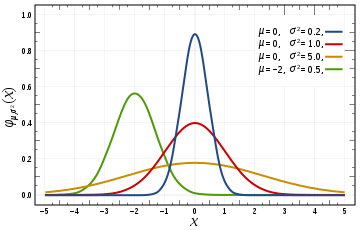
\includegraphics[width=\textwidth]{figures/gambar.png}
        \caption{.}
        \label{fig:fourth_nocaption}
    \end{subfigure}
    \caption{無子圖標題範例}
    \label{fig:four_nocaption}
\end{figure}
